\documentclass[a4paper,12pt]{article}
\usepackage{amsmath}
\usepackage{amssymb}
\usepackage[polish]{babel}
\usepackage{polski}
\usepackage[utf8]{inputenc}
\usepackage{indentfirst}
\usepackage{geometry}
\usepackage{array}
\usepackage[pdftex]{color,graphicx}
\usepackage{subfigure}
\usepackage{afterpage}
\usepackage{setspace}
\usepackage{color}
\usepackage{wrapfig}
\usepackage{listings}
\usepackage{datetime}
\usepackage[outdir=./]{epstopdf}

\renewcommand{\onehalfspacing}{\setstretch{1.6}}

\geometry{tmargin=2.5cm,bmargin=2.5cm,lmargin=2.5cm,rmargin=2.5cm}
\setlength{\parindent}{1cm}
\setlength{\parskip}{0mm}

\newenvironment{lista}{
\begin{itemize}
  \setlength{\itemsep}{1pt}
  \setlength{\parskip}{0pt}
  \setlength{\parsep}{0pt}
}{\end{itemize}}

\newcommand{\linia}{\rule{\linewidth}{0.4mm}}

\definecolor{lbcolor}{rgb}{0.95,0.95,0.95}
\lstset{
    backgroundcolor=\color{lbcolor},
    tabsize=4,
  language=C++,
  captionpos=b,
  tabsize=3,
  frame=lines,
  numbers=left,
  numberstyle=\tiny,
  numbersep=5pt,
  breaklines=true,
  showstringspaces=false,
  basicstyle=\footnotesize,
  identifierstyle=\color{magenta},
  keywordstyle=\color[rgb]{0,0,1},
  commentstyle=\color{Darkgreen},
  stringstyle=\color{red}
  }

\begin{document}

\noindent
\begin{tabular}{|c|p{11cm}|c|} \hline 
Grupa 1 & Kordian Kurdziel, Mateusz Maciejak & \ddmmyyyydate\today \tabularnewline
\hline 
\end{tabular}


\section*{Zadanie 3 - Rozmycie Gaussa w CUDA}

Celem zadania było stworzenie programu rozmywającego podane na wejściu obrazu, za pomocą algorytmu Gaussa z maską 5x5. Do zrównoleglenia obliczeń należało wykorzystać technologię CUDA.


\begin{lstlisting}
    cudaMalloc<unsigned char> (&cudaSrcImage, totalImageSize);
    cudaMalloc<unsigned char> (&cudaOutImage, totalImageSize);

    cudaMemcpy(cudaSrcImage, inputImg.ptr(), totalImageSize, cudaMemcpyHostToDevice);

    dim3 dimGrid = dim3(GRID_SIZE);
    dim3 dimBlock = dim3(BLOCK_SIZE);

    cudaEventCreate(&startEvent);
    cudaEventCreate(&endEvent);

    cudaEventRecord(startEvent, NULL);
    gaussianBlurCuda<<<dimGrid, dimBlock>>>(cudaSrcImage, cudaOutImage, inputImg.rows, rowLengthInBytes, inputImg.channels());
    cudaEventRecord(endEvent, NULL);
    cudaEventSynchronize(endEvent);
    cudaEventElapsedTime(&elapsedTime, startEvent, endEvent);

    cudaMemcpy(outputImg.ptr(), cudaOutImage, totalImageSize, cudaMemcpyDeviceToHost);
\end{lstlisting}

Na powyższym fragmencie kodu widać wykorzystanie API Cudy.

\begin{lstlisting}
 int col = (byteCounter % rowSizeInBytes) / channelsSize;

        if (byteCounter < 2 * rowSizeInBytes) continue;
        if (byteCounter > totalImageSize - 2 * rowSizeInBytes) continue;

        if (col < 2) continue;
        if (col >= (rowSizeInBytes / channelsSize) - 2) continue;

        int sum = 0;
    
        for (int i = 0; i < 5; i++)
        {
            for (int j = 0; j < 5; j++)
            {
                sum += globalMask[i][j] * imageSrc[byteCounter + (i - 2) * rowSizeInBytes + (j - 2) * channelsSize];
            }
        }           
        imageOut[byteCounter] = (int) (sum / deviceMaskWeight);

\end{lstlisting}

Powyższy listing przedstawia kod kernela, wykonywany równolegle przez wiele wątków na GPU.

\begin{figure}[!ht]
	\centering
  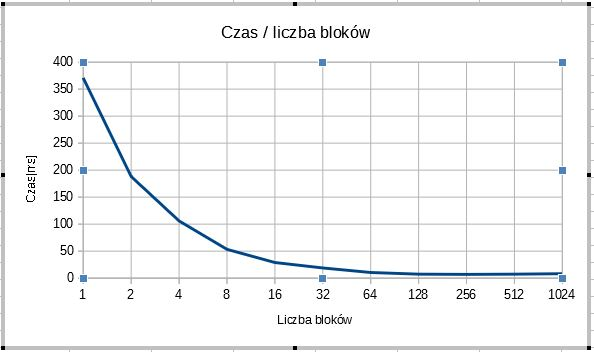
\includegraphics[width=0.9\textwidth]{wykresCzas.jpg}
  \caption{Wykres zależności czasu wykonywania obliczeń od liczby bloków}
\end{figure}

\begin{figure}[!ht]
	\centering
  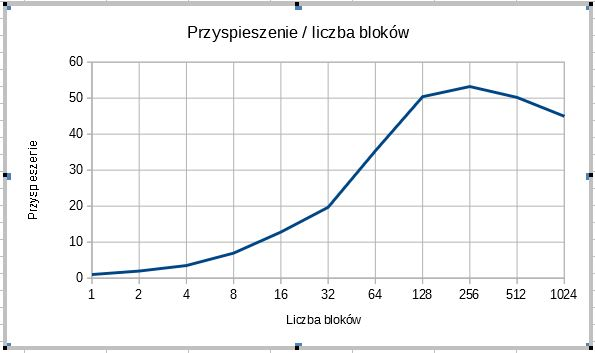
\includegraphics[width=0.9\textwidth]{wykresPrzyspieszenie.jpg}
  \caption{Wykres przyspieszenia działania programu w zależności od liczby bloków}
\end{figure}


Obliczenia wykonywane były na uczelnianym serwerze. Do testów używano obrazka w rozdzielczości 4K. Jak widać na podstawie wykresów, dzięki wykorzystaniu technologii CUDA, można wykorzystać moc kart obliczeniowych. Ich architektura sprawia, że są one wręcz idealne do pracy nad zadaniami, w których istotnym problemem są takie same, proste obliczenia wykonywane wielokrotnie na olbrzymim zbiorze danych.

\end{document}
